\chapter{基本类型}\label{ch03}
\emph{这个世界上有很多很多不同类型的书,这是一件好事。但也有很多很多不同类型的人,每个人都想读到一些不同的东西。}
\begin{flushright}
    ——Lemony Snicket
\end{flushright}

在很大程度上,Rust语言是围绕它的类型来设计的。它对高性能代码的支持源于让开发者选择不同情况下最合适的数据表示,并在简单性和成本之间取得适当的平衡。Rust的内存和线程安全也依赖于类型系统的健全性,Rust的灵活性则来自于它的泛型和trait。

这一章将介绍Rust的基本类型。这些源码级别的类型都有对应的成本和性能可预测的机器级的组件。尽管Rust并不保证它会完全按照你的要求精确的表示数据,但只有当它是一个可靠的改进时它才会违背你的要求。

与JavaScript或Python这种动态类型语言相比,Rust要求你事先就进行更多规划。你必须写出函数参数和返回值、结构体字段、以及一些其他结构的类型。然而,Rust的两个特性使得这比你想象中的要简单很多:

\begin{itemize}
    \item 有了你指明的类型,Rust的\emph{类型推导}将会为你推导出剩余的大部分类型。在实践中,通常只有一个类型能够满足给定的变量或表达式。在这种情况下,Rust允许你留空,或者说\emph{省略}这个类型。例如,你可以像下面这样写出一个函数里的所有类型:
          \begin{minted}{Rust}
    fn build_vector() -> Vec<i16> {
        let mut v: Vec<i16> = Vec::<i16>::new();
        v.push(10i16);
        v.push(20i16);
        v
    }
    \end{minted}
          但这非常杂乱和重复。给定了函数的返回值之后,很明显\texttt{v}必须是\texttt{Vec<i16>}类型:一个16位有符号整数的vector,没有其他的类型可以满足语义。并且据此可以推出vector的每个元素必须是\texttt{i16}类型。这就是Rust的类型推导适用的场景,所以你可以改为:
          \begin{minted}{Rust}
    fn build_vector() -> Vec<i16> {
        let mut v = Vec::new();
        v.push(10);
        v.push(20);
        v
    }
    \end{minted}
          这两个定义是完全等价的,Rust将会生成完全相同的机器代码。类型推导可以回馈一部分动态类型语言的可读性,并且仍能在编译时捕捉到类型错误。
    \item 函数可以是\emph{泛型}的:一个函数可以同时处理很多不同类型的值。

          在Python和JavaScript中,所有的函数都很自然的是泛型的:一个函数可以操作任何类型的值,只要这个类型有函数体中需要的属性和方法。(这种特性通常被称作\emph{鸭子类型}:如果它像鸭子一样叫,那它就是一只鸭子。)但正是这种灵活性也导致这些语言很难检测出类型错误,在这些语言里测试通常是唯一一种捕捉类型错误的方式。Rust的泛型函数给予了这门语言某种程度上和动态类型同样的灵活性,并且仍能在编译期捕获所有的类型错误。

          除了灵活性之外,泛型函数和非泛型的函数一样高效。例如,为每个整数类型都编写一个\texttt{sum}函数与编写一个处理所有整数类型的泛型\texttt{sum}函数相比,并没有性能上的优势。我们将在\hyperref[ch11]{第11章}种详细讨论泛型函数。
\end{itemize}

这一章的剩余部分将会自上而下的覆盖Rust的类型,从最简单的数字类型例如证书和浮点数到持有多个值的复合类型:box、tuple、数组和字符串。

这里有一个Rust中类型的汇总。\hyperref[t3-1]{表3-1}显示了Rust的原始类型,包括一些来自标准库的基本类型,和一些用户自定义类型的示例。

\begin{longtable}{p{0.25\textwidth}p{0.4\textwidth}p{0.25\textwidth}}
    \caption{Rust中的类型示例}
    \label{t3-1}\\
    \hline
    \textbf{类型}   & \textbf{描述}    & \textbf{值}    \\
    \hline
    \texttt{i8, i16, i32, i64, i128, u8, u16, u32, u64, u128}    & 指定位数的有符号和无符号整数 & \texttt{42, -5i8, 0x400u16, 0o100i16, 20\_922\_789\_888\_000u64, b'*'(u8字节字面量)}    \\
    \rowcolor{tablecolor}
    \texttt{isize, usize}   & 有符号和无符号整数,和机器里的一个指针一样大(32位或64位)   & \texttt{137, -0b0101\_0010isize, 0xffff\_fc00usize} \\
    \texttt{f32, f64}       & IEEE浮点数,单精度和双精度                                & \texttt{1.61803, 3.14f32, 6.0221e23f64} \\
    \rowcolor{tablecolor}
    \texttt{bool}           & 布尔值            & \texttt{true, false} \\
    \texttt{char}           & Unicode字符,32位 & \texttt{'*', '\textbackslash n', '字', '\textbackslash x7f', '\textbackslash u\{CA0\}'} \\
    \rowcolor{tablecolor}
    \texttt{(char, u8, i32)}                        & Tuple:把类型混合在一起   & \texttt{('\%', 0x7f, -1)} \\
    \texttt{()}                                     & “单元值”(空tuple)      & \texttt{()} \\
    \rowcolor{tablecolor}
    \texttt{struct S \{ x: f32, y: f32 \}}          & 命名字段结构体            & \texttt{S \{ x: 120.0, y: 209.0 \}} \\
    \texttt{struct T (i32, char);}                  & 元组结构体                & \texttt{T(120, 'X')} \\
    \rowcolor{tablecolor}
    \texttt{struct E;}                              & 元组结构体,无字段        & \texttt{E} \\
    \texttt{enum Attend \{ OnTime, Late(u32) \}}    & 枚举,代数数据类型        & \texttt{Attend::Late(5), Attend::OnTime} \\
    \rowcolor{tablecolor}
    \texttt{Box<Attend}                             & Box:持有一个堆上的值的指针   & \texttt{Box::new(Late(15))} \\
    \texttt{\&i32, \&mut i32}                       & 共享和可变引用:生命周期不能超过所引用对象的无所有权的指针 & \texttt{\&s.y, \&mut v} \\
    \rowcolor{tablecolor}
    \texttt{String}                                 & UTF-8字符串,动态大小         & \texttt{"ラーメン: ramen"\newline.to\_string()} \\
    \texttt{\&str}                                  & \texttt{str}的引用:指向UTF-8字符串的无所有权的指针 & \texttt{"そば: soba", \&s[0..12]} \\
    \rowcolor{tablecolor}
    \texttt{[f64; 4], [u8; 256]}                    & 固定长度的数组,所有元素的类型都必须相同   & \texttt{[1.0, 0.0, 0.0, 1.0], [b' '; 256]} \\
    \texttt{Vec<f64>}                               & 可变长度的vector,所有元素的类型都必须相同 & \texttt{vec![0.367, 2.718, 7.389]} \\
    \rowcolor{tablecolor}
    \texttt{\&[u8], \&mut [u8]}                     & 切片的引用:指向数组或vector的一部分,包含指针和长度 & \texttt{\&v[10..20], \&mut a[..]} \\
    \texttt{Option<\&str>}      & 可选值:\texttt{None}(无值)或\texttt{Some(v)}(有值,值为\texttt{v})   & \texttt{Some("Dr.", None)} \\
    \rowcolor{tablecolor}
    \texttt{Result<u64, Error>} & 可能会失败的操作的结果:成功时是\texttt{Ok(v)},失败时是\texttt{Err(e)} & \texttt{Ok(4096), Err(Error::last\_os\_error())} \\
    \texttt{\&dyn Any, \&mut dyn Read}  & trait对象:指向一个实现了给定方法的任何值 & \texttt{value as \&dyn Any, \&mut file as \&mut dyn Read} \\
    \rowcolor{tablecolor}
    \texttt{fn(\&str) -> bool}          & 函数指针      & \texttt{str::is\_empty}           \\
    (闭包类型)                         & 闭包         & \texttt{|a, b| \{ a*a + b*b \}}    \\
\end{longtable}

这些类型中的大部分都会在这一章中介绍,除了下面这些:
\begin{itemize}
    \item 我们将在\hyperref[ch09]{第9章}中单独介绍\texttt{struct}类型。
    \item 我们将在\hyperref[ch10]{第10章}中单独介绍枚举类型。
    \item 我们将在\hyperref[ch11]{第11章}中介绍trait对象。
    \item 我们将在这里介绍\texttt{String}和\texttt{\&str}的基础,但在\hyperref[ch17]{第17章}中介绍更多细节。
    \item 我们将在\hyperref[ch14]{第14章}介绍函数和闭包类型。
\end{itemize}

\section{固定位数的数字类型}
Rust类型系统的基础是一组固定宽度的数字类型的集合,这些类型和现代处理器中的硬件类型相匹配。

固定宽度的数字类型可能会溢出或失去精度,但它们适用于大多数的类型,并且比任意精度的整数和精确小数快几千倍。如果你需要那些类型的数字,可以在\texttt{num} crate找到相应的支持。

Rust的数字类型的名称遵循通用的模式,宽度加上表示的含义(\hyperref[f3-2]{表3-2})。
\begin{table}[htbp]
    \centering
    \caption{Rust的数字类型}
    \label{f3-2}
    \begin{tabular}{llll}
        \hline
        \textbf{大小(比特数)}   & \textbf{无符号整数}   & \textbf{有符号整数}   & \textbf{浮点数}   \\
        \hline
        \texttt{8}  & \texttt{u8}   & \texttt{i8}   &              \\
        \rowcolor{tablecolor} 
        \texttt{16} & \texttt{u16}  & \texttt{i16}  &              \\
        \texttt{32} & \texttt{u32}  & \texttt{i32}  & \texttt{f32} \\
        \rowcolor{tablecolor} 
        \texttt{64} & \texttt{u64}  & \texttt{i64}  & \texttt{f64} \\
        \texttt{128}& \texttt{u128} & \texttt{i128} &              \\
        \rowcolor{tablecolor} 
        机器字      & \texttt{usize} & \texttt{isize} & \\
    \end{tabular}
\end{table}

这里,\emph{机器字}是运行代码的机器上的一个指针的大小,32位或者64位。

\subsection{整数类型}

Rust的无符号整数使用全部的范围来表示正数和0(\hyperref[t3-3]{表3-3})。
\begin{table}[htbp]
    \centering
    \caption{Rust无符号整数类型}
    \label{t3-3}
    \begin{tabular}{ll}
        \hline
        \textbf{类型}   &   \textbf{范围}                   \\
        \hline
        \texttt{u8}     & 0到$2^{8}-1$(0到255)            \\
        \rowcolor{tablecolor} 
        \texttt{u16}    & 0到$2^{16}-1$(0到65,535)        \\
        \texttt{u32}    & 0到$2^{32}-1$(0到4,294,967,295) \\
        \rowcolor{tablecolor} 
        \texttt{u64}    & 0到$2^{64}-1$(0到18,446,744,073,709,551,615或1万8千亿)  \\
        \texttt{u128}   & 0到$2^{128}-1$(0到大约$3.4*10^{38}$)                    \\
        \rowcolor{tablecolor} 
        \texttt{usize}  & 0到$2^{32}-1$或$2^{64}-1$         \\
    \end{tabular}
\end{table}

Rust的有符号整数使用两种互补的表示方法,使用和无符号类型相对应的位模式来表示一个包含正数和负数的范围(\hyperref[t3-4]{表3-4})。
\begin{table}[htbp]
    \centering
    \caption{Rust的有符号整数类型}
    \label{t3-4}
    \begin{tabular}{ll}
        \hline
        \textbf{类型}   &   \textbf{范围}   \\
        \hline
        \texttt{i8}     & $-2^{7}$到$2^{7}-1$(-128到127)   \\
        \rowcolor{tablecolor}
        \texttt{i16}    & $-2^{15}$到$2^{15}-1$(-32,768到32,767)  \\
        \texttt{i32}    & $-2^{31}$到$2^{31}-1$(-2,147,483,648到2,147,483,647)    \\
        \rowcolor{tablecolor}
        \texttt{i64}    & $-2^{63}$到$2^{63}-1$(-9,223,372,036,854,775,808到9,223,372,036,854,775,807)    \\
        \texttt{i128}   & $-2^{127}$到$2^{127-1}$(大约$-1.7\times10^{38}$到$+1.7\times10^{38}$) \\
        \rowcolor{tablecolor}
        \texttt{isize}  & $-2^{31}$到$2^{31}-1$,或者$-2^{63}$到$2^{63}-1$  \\
    \end{tabular}
\end{table}

Rust使用\texttt{u8}类型来表示一个字节的值。例如,从二进制文件或者套接字读取数据就会返回\texttt{u8}类型的数据流。

与C和C++不同,Rust区分了字符和数字类型:\texttt{char}不是\texttt{u8},也不是\texttt{u32}(尽管它是32位)。我们将会在“\hyperref[char]{字符}”这一节介绍Rust的\texttt{char}类型。

\texttt{usize}和\texttt{isize}类似于C和C++中的\texttt{size\_t}和\texttt{ptrdiff\_t}类型。它们的位数和目标机器上地址空间的位数相同:在32位架构上就是32位,在64位架构上就是64位。Rust要求数组索引为\texttt{usize}类型的值。数组或vector或其他任何含有多个元素的数据结构的长度都是\texttt{usize}类型。

Rust中的整数字面量可以有一个后缀来指示类型:\texttt{42u8}是一个\texttt{u8}类型的值,\texttt{1729isize}是一个\texttt{isize}类型的值。如果一个整数字面量没有类型后缀,Rust将会延迟决定它的类型,直到可以从它的使用中推断出它的类型:存储到一个已知类型的变量中、作为参数传递给一个参数类型已知的函数、和一个已知类型的值比较、以及类似的情况。如果到最后还是有很多类型可以满足,此时如果\texttt{i32}是其中一种可能,Rust将推断它为\texttt{i32}类型。否则,Rust会报歧义错误。

前缀\texttt{0x, 0o, 0b}分别表示十六进制、八进制、二进制字面量。

为了让长数字更更读,你可以在数字中间插入下划线。例如,你可以把最大的\texttt{u32}值写作\texttt{4\_294\_967\_295}。下划线放置的位置并不重要,所以你可以每四位插入一个下划线来把十六进制和二进制数字分组,例如\texttt{0xffff\_ffff}或者在最后插入下划线分隔类型后缀,例如\texttt{127\_u8}。\hyperref[t3-5]{表3-5}给出了一些整数字面量的例子。
\begin{table}[htbp]
    \centering
    \caption{整数字面量的例子}
    \label{t3-5}
    \begin{tabular}{lll}
        \hline
        \textbf{字面量} & \textbf{类型} & \textbf{十进制值} \\
        \hline
        \texttt{116i8}          & \texttt{i8}       &   116 \\
        \rowcolor{tablecolor}
        \texttt{0xcafeu32}      & \texttt{u32}      &   51966 \\
        \texttt{0b0010\_1010}   & 推断              &   42 \\
        \rowcolor{tablecolor}
        \texttt{0o106}          & 推断              &   70 \\
    \end{tabular}
\end{table}

尽管数值类型和\texttt{char}类型是不同的,Rust确实提供了\emph{字节字面量}:很像字符字面量的\texttt{u8}值:\texttt{b'X'}代表字符\texttt{X}的ASCII码值,但是是\texttt{u8}类型的值。例如,因为\texttt{A}的ASCII码值是65,字面量\texttt{b'A'}和\texttt{65u8}是等价的。只有ASCII字符可以出现在字节字面量中。

这里有一些不能用单个字符表示的字符,因为它们要么会导致歧异要么很难看出来。\hyperref[t3-6]{表3-6}中的字符只能用反斜杠转移的方式写出来。
\begin{table}[htbp]
    \centering
    \caption{需要转义的字符}
    \label{t3-6}
    \begin{tabular}{lll}
        \hline
        \textbf{字符}   &   \textbf{字节字面量} & \textbf{等价的数字值} \\
        \hline
        单引号,'   &   \texttt{b'\textbackslash''}      & 39u8 \\
        \rowcolor{tablecolor}
        反斜杠,\textbackslash &    \texttt{b'\textbackslash\textbackslash'} & 92u8 \\
        换行        &    \texttt{b'\textbackslash n'}    & 10u8 \\
        \rowcolor{tablecolor}
        回车        &   \texttt{b'\textbackslash r'}     & 13u8 \\
        制表符      &   \texttt{b'\textbackslash t'}     & 9u8 \\
    \end{tabular}
\end{table}

对于那些难以写出或看出的字符,你可以用它们的十六进制码代替。一个字节字面量的形式是\texttt{b'\textbackslash xHH'},其中\texttt{HH}是两个十六进制的数字,代表值是\texttt{HH}的字节。例如,你可以将ASCII的“escape”字符的字节字面量写作\texttt{b'\textbackslash x1b'},因为“escape”的ASCII码是27,也就是16进制的1B。因为字节字面量只是\texttt{u8}类型值的另一种表示方式,考虑使用数字字面量可能可读性会更强:只有当你想表示ASCII码时\texttt{b'\textbackslash x1b'}才会比\texttt{27}更有意义。

你可以将一种整数类型转换为另一种整数类型。我们将会在“\hyperref[cast]{类型转换}”这一节中介绍转换的原理,这里有一些例子:
\begin{minted}{Rust}
    assert_eq!(   10_i8  as u16,    10_u16); // in range
    assert_eq!( 2525_u16 as i16,  2525_i16); // in range

    assert_eq!(   -1_i16 as i32,    -1_i32); // 符号扩展
    assert_eq!(65535_u16 as i32, 65535_i32); // 0扩展

    // 转换一个超出目标类型范围的值
    // 等价于原值对2^N取模
    // N是目标类型的位数
    // 这有时也被称为“截断”
    assert_eq!( 1000_i16 as  u8,    232_u8);
    assert_eq!(65535_u32 as i16,     -1_i16);

    assert_eq!(   -1_i8  as u8,     255_u8);
    assert_eq!(  255_u8  as i8,      -1_i8);
\end{minted}

标准库提供一些整数的方法来进行操作。例如:
\begin{minted}{Rust}
    assert_eq!(2_u16.pow(4), 16);               // 求指数幂
    assert_eq!((-4_i32).abs(), 4);              // 求绝对值
    assert_eq!(0b101101_u8.count_ones(), 4);    // 位计数
\end{minted}

你可以在在线文档中找到这些。但是注意,文档中\texttt{i32}(原始类型)和模块导入的类型(搜索\texttt{std::i32})有不同的单独页面。

在实际编码时,你不需要像我们在这里一样写出类型后缀,因为上下文会自动推断出类型。当推断不出来时,错误信息可能会让你很惊讶。例如,下面的代码不能编译:
\begin{minted}{Rust}
    println!("{}", (-4).abs());
\end{minted}

Rust报错:
\begin{minted}{text}
    error: can't call method `abs` on ambiguous numeric type `{integer}`
\end{minted}

这可能有点迷惑:所有的整数类型都有\texttt{abs}方法,所以问题在哪呢?从技术角度来说,Rust需要在调用某个类型的方法之前知道这个值的精确类型。只有当所有的方法调用都被解析之后仍然存在歧义才会使用默认的\texttt{i32}类型,而在这里,在解析\texttt{abs}方法时就需要知道\texttt{-4}的类型,默认推导为\texttt{i32}的规则在此时不能生效。解决方法是指明类型,要么加上类型后缀,要么使用类型特定的函数:
\begin{minted}{Rust}
    println!("{}", (-4_i32).abs());
    println!("{}", i32::abs(-4));
\end{minted}

注意函数调用的优先级高于一元前缀运算符,所以当对负数调用方法时一定要小心。如果这个地方第一个表达式里\texttt{-4\_i32}两侧没有括号,\texttt{-4\_i32.abs()}将会对\texttt{4}调用\texttt{abs}方法,返回正数\texttt{4},然后求负数返回\texttt{-4}。

\subsection{Checked、Wrapping、Saturating、Overflowing算术}

当整数运算溢出时,如果是在debug模式下Rust会panic。在release模式下,运算结果会\emph{回环}:它会返回正确的值对结果类型能表示的范围取余之后的结果。(这两种情况下,溢出都不像在C和C++中一样是未定义行为)。

例如,下面的代码在debug模式下会panic:
\begin{minted}{Rust}
    let mut i = 1;
    loop {
        i *= 10;    // panic: 尝试乘到溢出
                    // (但只有在debug模式会panic!)
    }
\end{minted}

在release模式下,溢出时乘法会回环成负数,然后循环会无限执行。

如果默认行为不是你希望的结果,整数类型提供了一个方法让你指定想要做什么。例如,下面的代码在任何构建模式下都会panic:
\begin{minted}{Rust}
    let mut i: i32 = 1;
    loop {
        // panic: 乘法溢出(在任何构建模式下)
        i = i.checked_mul(10).expect("multiplication overflowed");
    }
\end{minted}

这些整数运算的方法可以被分为四个通用的类别:
\begin{itemize}
    \item \emph{Checked}操作返回一个结果的\texttt{Option}值:如果运算结果可以被结果类型正确表示就返回\texttt{Some(v)},否则返回\texttt{None}。例如:
    \begin{minted}{Rust}
    // 10和20的结果可以用u8表示。
    assert_eq!(10_u8).checked_add(20), Some(30));

    // 不幸的是,100和200的和不能用u8表示。
    assert_eq!(100_u8).checked_add(200), None);

    // 求和,如果溢出就panic。
    let sum = x.checked_add(y).unwrap();

    // 奇怪的是,在一种特定情况下,有符号除法也可能会导致溢出。
    // 一个有符号整数能表示-2^(n-1),但不能表示2^(n-1)。
    assert_eq!((-128_i8).checked_div(-1), None);
    \end{minted}

    \item \emph{Wrapping}操作返回正确的值对结果类型能表示的范围的余数:
    \begin{minted}{Rust}
    // 第一个积可以用u16来表示。
    // 第二个不能,因此我们得到250000对2^16取模。
    assert_eq!(100_u16.wrapping_mul(200), 20000);
    assert_eq!(500_u16.wrapping_mul(500), 53392);

    // 有符号数的操作可能会回环成负数。
    assert_eq!(500_i16.wrapping_mul(500), -12144);

    // 在移位操作中,移动的位数会回环到该类型的位数之内
    // 因此对16位的数字移动17位等于移动1位
    assert_eq!(5_i16.wrapping_shl(17), 10);
    \end{minted}
    正如解释的那样,这就是release模式下算术操作的行为。使用这种写法的好处是在所有的构建模式下代码的行为都一致。

    \item \emph{Saturating}操作会返回最接近正确结果的表示。换句话说,结果被“截断”到这个类型能表示的最大或最小值:
    \begin{minted}{Rust}
    assert_eq!(32760_i16.saturating_add(10), 32767);
    assert_eq!((-32760_i16).saturating_sub(10), -32768);
    \end{minted}
    没有饱和除法、取余、位移操作。

    \item \emph{Overflowing}操作返回一个tuple\texttt{(reulst, overflowed)},其中\texttt{result}是回环版本的方法返回的结果,而\texttt{overflowed}是一个指示是否发生溢出的\texttt{bool}值:
    \begin{minted}{Rust}
    assert_eq!(255_u8.overflowing_sub(2), (253, false));
    assert_eq!(255_u8.overflowing_add(2), (1, true));
    \end{minted}
    \texttt{overflowing\_shl}和\texttt{overflowing\_shr}稍微有些偏离这个模式:只有当移位距离恰好等于类型的位宽度时\texttt{overflowed}才为true。实际的移位距离等于要求的距离对位宽度取余后的结果:
    \begin{minted}{Rust}
    // 对`u16`来说移动17位太多了,17对16取余等于1。
    assert_eq!(5_u16.overflowing_shl(17), (10, true));
    \end{minted}
\end{itemize}

\hyperref[t3-7]{表3-7}中列出了以\texttt{checked\_},\texttt{wrapping\_},\texttt{saturating\_},\texttt{overflowing\_}为前缀的方法。
\begin{table}[htbp]
    \centering
    \caption{操作的名称}
    \label{t3-7}
    \begin{tabular}{lll}
        \hline
        \textbf{操作}   & \textbf{名称后缀} &   示例 \\
        \hline
        加法    &   \texttt{add}    & \texttt{100\_i8.checked\_add(27) == Some(127)}    \\
        \rowcolor{tablecolor}
        减法    &   \texttt{sub}    & \texttt{10\_u8.checked\_sub(11) == None}      \\
        乘法    &   \texttt{mul}    & \texttt{128\_u8.saturating\_mul(3) == 255}    \\
        \rowcolor{tablecolor}
        除法    &   \texttt{div}    & \texttt{64\_u16.wrapping\_div(8) == 8}    \\
        取余    &   \texttt{rem}    & \texttt{(-32768\_i16).wrapping\_rem(-1) == 0} \\
        \rowcolor{tablecolor}
        负数    &   \texttt{neg}    & \texttt{(-128\_i8).checked\_neg() == None} \\
        绝对值  &   \texttt{abs}    & \texttt{(-32768\_i16).wrapping\_abs() == -32768} \\
        \rowcolor{tablecolor}
        指数    &   \texttt{pow}    & \texttt{3\_u8.checked\_pow(4) == Some(81)} \\
        左移    &   \texttt{shl}    & \texttt{10\_u32.wrapping\_shl(34) == 40}  \\
        \rowcolor{tablecolor}
        右移    &   \texttt{shr}    & \texttt{40\_u64.wrapping\_shr(66) == 10}  \\
    \end{tabular}
\end{table}

\subsection{浮点数}
Rust提供IEEE的单精度和双精度浮点数。这两个类型还包括正无穷、负无穷、正0、负0和\emph{非数}值。(\hyperref[t3-8]{表3-8})

\begin{table}[htbp]
    \centering
    \caption{IEEE单精度和双精度浮点数类型}
    \label{t3-8}
    \begin{tabular}{lll}
        \hline
        \textbf{类型}   & \textbf{精度} &   \textbf{范围}   \\
        \hline
        \texttt{f32}    & IEEE单精度浮点数(至少6位十进制数字)    & 大约$-3.4\times10^{38}$到$+3.4\times10^{38}$    \\
        \rowcolor{tablecolor}
        \texttt{f64}    & IEEE双精度浮点数(至少15位十进制数字)    & 大约$-1.8\times10^{308}$到$1.8\times10^{308}$   \\
    \end{tabular}
\end{table}

Rust的\texttt{f32}和\texttt{f64}分别对应C和C++(如果实现支持IEEE浮点数的话)以及Java(总是使用IEEE浮点数)里的\texttt{float}和\texttt{double}类型。

浮点数字面量的一般形式如\hyperref[f3-1]{图3-1}。
\begin{figure}[htbp]
    \centering
    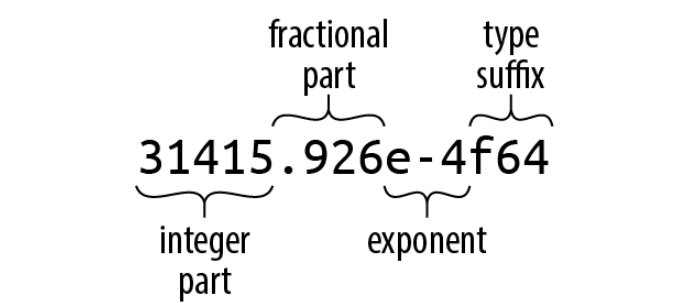
\includegraphics[width=0.8\textwidth]{../img/f3-1.png}
    \caption{浮点数字面量}
    \label{f3-1}
\end{figure}

整数部分之后的部分都是可选的,但小数部分、指数、或者类型后缀至少需要有一个,才能和整数字面量区分开。小数部分可以只有一个单独的小数点,因此\texttt{5.}是一个有效的浮点数。

如果一个浮点数字面量缺少类型后置,和处理整数一样,Rust会检查上下文来查看这个值是如何使用的。如果最后它发现两种浮点数类型都可以满足语义,那么它会默认选择\texttt{f64}。

为了实现类型推导,Rust把整数字面量和浮点数字面量区分为不同的种类:它从来不会把一个浮点数类型推断为整数类型,反之亦然。\hyperref[t3-9]{表3-9}展示了一下浮点数字面量的例子。

\begin{table}[htbp]
    \centering
    \caption{浮点数字面量的示例}
    \label{t3-9}
    \begin{tabular}{lll}
        \hline
        \textbf{字面量} & \textbf{类型} & \textbf{数值} \\
        \hline
        \texttt{-1.5625}    & 自动推断  & $-1\frac{9}{16}$  \\
        \rowcolor{tablecolor}
        \texttt{2.}         & 自动推断  & 2 \\
        \texttt{0.25}       & 自动推断  & $\frac{1}{4}$   \\
        \rowcolor{tablecolor}
        \texttt{1e4}        & 自动推断  & 10,000    \\
        \texttt{40f32}      & \texttt{f32}  & 40    \\
        \rowcolor{tablecolor}
        \texttt{9.109\_383\_56e-31f64} & \texttt{f64} & 大约是$9.10938356\times10^{-31}$ \\
    \end{tabular}
\end{table}

\texttt{f32}和\texttt{f64}类型还关联了IEEE要求的特殊常量值例如\texttt{INFINITY}、\texttt{NEG\_INFINITY}(负无穷)、\texttt{NAN}(非数值)、\texttt{MIN}和\texttt{MAX}(最小和最大的有限值):
\begin{minted}{Rust}
    assert!((-1. / f32::INFINITY).is_sign_negative());
    assert_eq!(-f32::MIN, f32::MAX);
\end{minted}
\texttt{f32}和\texttt{f64}类型提供了完整的数值计算的方法;例如,\texttt{2f64.sqrt()}是2的平凡根。还有一些示例:
\begin{minted}{Rust}
    assert_eq!(5f32.sqrt() * 5f32.sqrt(), 5.);  // 精确的5.0
    assert_eq!((-1.01f64).floor(), -2.0);
\end{minted}

再重复一次,方法调用的优先级高于前缀运算符,因此对负数调用方法时确保要用括号括起来。

\texttt{std::f32::consts}和\texttt{std::f64::consts}模块提供了常用的数学常数,例如\texttt{E}、\texttt{PI}、2的平方根。

当查找文档时,记得既有类型的文档,名称叫“\texttt{f32}(primitive type)”和“\texttt{f64}(primitive type)”,又有模块的文档,名称叫\texttt{std::f32}和\texttt{std::f64}。

和整数一样,在实际编码时通常你不需要写出浮点数字面量的类型后缀,但如果你要写,那么只需要指明变量和函数其中一个类型即可:
\begin{minted}{Rust}
    println!("{}", (2.0_f64).sqrt());
    println!("{}", f64::sqrt(2.0));
\end{minted}
和C和C++不同,Rust中几乎没有隐式类型转换。如果一个函数接收\texttt{f64}类型的参数,传递\texttt{i32}的值作为参数将是一个错误。事实上,Rust甚至不允许从\texttt{i16}到\texttt{i32}这样的隐式转换,尽管每一个\texttt{i16}值也都是一个合法的\texttt{i32}值。但你总是可以使用\texttt{as}运算符来进行\texttt{显式}转换:\texttt{i as f64},或者\texttt{x as i32}。

缺少隐式类型转换导致Rust的表达式可能会比C和C++中类似的表达式更加冗长。然而,隐式整数转换经常导致bug和安全漏洞。尤其是用来表示内存中某个东西的长度的整数,可能会导致意外的溢出。在我们的实践中,在Rust中显式写出类型转换可以提醒我们可能忽略的问题。

我们会在“\hyperref[cast]{类型转换}”一节中介绍转换的原理。

\section{布尔类型}

Rust的布尔类型\texttt{bool},只有两个值:\texttt{true}和\texttt{false}。比较运算符例如\texttt{==}和\texttt{<}会产生\texttt{bool}类型的结果:\texttt{2 < 5}的结果是\texttt{true}。

许多语言都很宽容,允许在需要布尔值的上下文中使用其他类型:C和C++隐式把字符、整数、浮点数和指针转换为布尔值,因此它们可以直接用作\texttt{if}或\texttt{while}语句的条件。Python还允许string、list、字典、甚至集合用作布尔值,如果不为空时视为true。然而Rust非常严格:像\texttt{if}和\texttt{while}这样的控制流的条件必须是\texttt{bool}表达式,短路求职运算符\texttt{\&\&}和\texttt{||}也是这样。你必须写\texttt{if x != 0 \{ ... \}},而不能写\texttt{if x \{ ... \}}。

Rust的\texttt{as}运算符可以把\texttt{bool}值转换为整数值:
\begin{minted}{Rust}
    assert_eq!(false as i32, 0);
    assert_eq!(true  as i32, 1);
\end{minted}

然而,\texttt{as}不能反过来把整数值转换为\texttt{bool}值。你必须显式写出比较运算例如\texttt{x != 0}。

尽管\texttt{bool}类型只需要单个比特来表示,Rust还是使用整个字节来表示\texttt{bool},因此你可以创建指向它的指针。

\section{字符}\label{char}
Rust的字符类型\texttt{char}代表一个单独的Unicode字符,是一个32位的值。

Rust使用\texttt{char}表示单个字符,但使用UTF-8编码字符串和文本流。因此,\texttt{String}表示它的文本是一个UTF-8字节序列,而不是字符的数组。

字符串字面量是被单括号包围的单个字符,例如\texttt{'8'}或\texttt{'!'}。你可以使用Unicode范围内的任何字符:\texttt{'錆'}是一个\texttt{char}字面量代表日语汉字中的\emph{sabi}(rust)。

和字节字面量一样,一些字符需要反斜杠转义(\hyperref[t3-10]{表3-10})。
\begin{table}[htbp]
    \centering
    \caption{需要反斜杠转义的字符}
    \label{t3-10}
    \begin{tabular}{lll}
        \hline
        \textbf{字符}   &   \textbf{Rust字符字面量} \\
        \hline
        单引号,'   &   \texttt{b'\textbackslash''} \\
        \rowcolor{tablecolor}
        反斜杠,\textbackslash &    \texttt{b'\textbackslash\textbackslash'} \\
        换行        &    \texttt{b'\textbackslash n'} \\
        \rowcolor{tablecolor}
        回车        &   \texttt{b'\textbackslash r'} \\
        制表符      &   \texttt{b'\textbackslash t'} \\
    \end{tabular}
\end{table}

如果你喜欢的话,你可以以十六进制的方式写出一个字符的Unicode编码:
\begin{itemize}
    \item 如果字符的码点在U+0000道U+007F之间(可以据此判断是否在ASCII字符集之中),那么你可以将字符写作\texttt{'\textbackslash xHH'},\texttt{HH}是一个两位的十六进制数字。例如,字符字面量\texttt{'*'}和\texttt{'\textbackslash x2A'}是等价的,因为字符\texttt{*}的码点是42,十六进制是2A。
    \item 你可以用\texttt{'\textbackslash u{HHHHHH}'}形式写出任何Unicode字符,\texttt{HHHHHH}是一个最长6位的十六进制数字,可以用下划线分隔。\footnote{译者注:此处原文中给了一个例子,但译者不知道该怎么打出卡纳达语里的字符,复制粘贴也不行,就省略了这个例子。}
\end{itemize}

一个\texttt{char}总是存储一个在0x0000到0xD7FF或0xE000到0x10FFFF之间的Unicode码点。一个\texttt{char}绝不会在两个范围之间(即0xD800到0xDFFF),也不会超出Unicode的编码空间(即大于0x10FFFF)。Rust使用类型系统和动态检查来确保\texttt{char}值总是在允许的范围内。

Rust永远不会进行\texttt{char}和其他任何类型之间的隐式转换。你可以使用\texttt{as}转换运算符来把\texttt{char}转换为整数类型,对于小于32位的类型,字符值的高位会被截断:\footnote{译者注:这个例子中也省略了卡纳达语字符相关的内容}
\begin{minted}{Rust}
    assert_eq!('*' as i32, 42);
\end{minted}

插句题外话,\texttt{u8}是唯一可以用\texttt{as}运算符转换成\texttt{char}的整数类型:Rust认为这时的\texttt{as}运算开销很低并且不可能失败,但任何\texttt{u8}之外的整数类型都包含不是有效的Unicode码点的值,因此这些转换需要运行时检查。所以,标准库提供了函数\texttt{std::char::from\_u32}接受任何\texttt{u32}值,并返回\texttt{Option<char>}:如果\texttt{u32}的值不是合法的Unicode码点,\texttt{from\_u32}会返回\texttt{None};否则,它会返回\texttt{Some(c)},\texttt{c}就是作为转换结果的\texttt{char}。

标准库为字符类型提供了一些有用的方法,你可以在文档中的“\texttt{char}(primitive type)”和模块“\texttt{std::char}”的页面中查找这些方法。例如:
\begin{minted}{Rust}
    assert_eq!('*'.is_alphabetic(), false);
    assert_eq!('β'.is_alphabetic(), true);
    assert_eq!('8'.to\_digit(10), Some(8));
    assert_eq!(std::char::from_digit(2, 10), Some('2'));
\end{minted}

当然,单个字符显然没有字符串和文本流有趣。我们将会在“\hyperref[string]{字符串类型}”中介绍Rust的标准\texttt{String}类型和常用的文本处理操作。

\section{元组}
\emph{元组}是两个、或三个、四个、五个、……不同类型的值的组合。你可以将元组看作被逗号分隔和括号包围的元素序列。例如,\texttt{("Brazil", 1985)}是一个元组,它的第一个元素是一个静态分配的字符串,第二个元素是一个整数,它的类型是\texttt{(\&str, i32)}。给定一个元组值\texttt{t},你可以通过\texttt{t.0}、\texttt{t.1}、……来访问它的元素。

某种程度上,元组类似于数组:这两个类型都代表一系列有固定顺序的值。许多编程语言合并或结合了这两种概念,但在Rust中,它们是完全独立的。一方面,元组的每个元素可以拥有不同的类型,而数组的所有元素必须有相同的类型。另外,元组只允许常数索引,例如\texttt{t.4}。你不可能写\texttt{t.i}或者\texttt{t[i]}来获取第i个元素。

Rust代码中经常使用元组类型来返回多个值。例如,字符串切片中的\texttt{split\_at}方法:用于将一个字符串切分为两半并返回的函数,被声明为类似如下形式:
\begin{minted}{Rust}
    fn split_at(&self, mid: usize) -> (&str, &str);
\end{minted}

返回类型\texttt{(\&str, \&str)}是两个字符串切片组成的元组。你可以使用模式匹配语法来把返回的元素赋值给不同的变量:
\begin{minted}{Rust}
    let text = "I see the eigenvalue in thine eye";
    let (head, tail) = text.split_at(21);
    assert_eq!(head, "I see the eigenvalue ");
    assert_eq!(tail, "in thine eye");
\end{minted}

这比下边的等价代码可读性更强:
\begin{minted}{Rust}
    let text = "I see the eigenvalue in thine eye";
    let temp = text.split_at(21);
    let head = temp.0;
    let tail = temp.1;
    assert_eq!(head, "I see the eigenvalue ");
    assert_eq!(tail, "in thine eye");
\end{minted}

你也可以将元组视为一种极简的结构体类型。例如,在\hyperref[ch02]{第2章}的曼德勃罗集程序中,我们需要向函数传递要绘制的图片的宽度和高度。我们可以声明一个有\texttt{width}和\texttt{height}成员的结构体,但这么简单的事没有必要搞得这么复杂,因此我们用了一个元组:
\begin{minted}{Rust}
    /// 写入缓冲区`pixels`,它的大小由`bounds`给出,
    /// 写入的文件名是`filename`。
    fn write_image(filename: &str, pixels: &[u8], bounds: (usize, usize))
        -> Result<(), std::io::Error>
    { ... }
\end{minted}

参数\texttt{bounds}的类型是\texttt{(usize, usize)},一个有两个\texttt{usize}值得元组。诚然,我们可以直接使用单独的\texttt{width}和\texttt{height}参数,生成的机器代码也会完全相同。这么写的目的只是想表明,我们把图片的大小看成一个值,而不是两个值,使用元组的写法可以清晰的表现出这一点。

元组的另一个常见用法是0元组\texttt{()}。这通常被称为\emph{单元类型}因为它只有一个取值,也写作\texttt{()}。Rust在上下文要求某种类型,但没有有意义的值要传递的情况下使用单元类型。

例如,一个不返回值的函数的返回类型是\texttt{()}。标准库中的\texttt{std::mem::swap}函数没有有意义的返回值;它只是交换两个参数的值。\texttt{std::mem::swap}的声明如下:
\begin{minted}{Rust}
    fn swap<T>(x: &mut T, y: &mut T);
\end{minted}
\texttt{<T>}意味着\texttt{swap}是\emph{泛型}的:你可以将它用于任何类型\texttt{T}的引用。但签名中省略了\texttt{swap}的返回类型,这实际上是返回单元类型的缩写:
\begin{minted}{Rust}
    fn swap<T>(x: &mut T, y: &mut T) -> ();
\end{minted}

与此类似,我们之前提到的\texttt{write\_image}例子中返回值类型是\texttt{Result<(), std::io::Error>},这意味着如果出错时函数返回\texttt{std::io::Error}类型的值,如果成功时返回无值。

如果你想的话,你可以在元组的最后一个元素之后加上一个逗号:类型\texttt{(\&str, i32,)}和\texttt{(\&str, i32)}是等价的,\texttt{("Brazil", 1985,)}和\texttt{("Brazil", 1985)}也是。Rust允许任何逗号分隔的值列表最后加上一个额外的逗号:函数参数、数组、结构体和枚举定义,等等。这对人类来说可能看起来很奇怪,但当需要在最后添加或删除条目时会变得方便一些。

为了一致性,还有只包含单个值的元组。字面量\texttt{("lonely hearts",)}是一个包含单个字符串的元组,它的类型是\texttt{(\&str,)}。这里,最后的逗号是必须的,这是为了和单纯的用括号把表达式括起来相区分。

